\documentclass{article}
\usepackage[utf8]{inputenc}
\usepackage{float}
\usepackage{makecell}
\newcommand\tab[1][0.5cm]{\hspace*{#1}}
\newcommand{\N}{\mathbb{N}}
\usepackage{mathtools}
\usepackage{amssymb}
\usepackage{todonotes}
\usepackage{hyperref}

\usepackage{amsfonts}

\usepackage{czech}

\oddsidemargin=-5mm
\evensidemargin=-5mm\marginparwidth=.08in \marginparsep=.01in
\marginparpush=5pt\topmargin=-15mm
\textwidth=17cm\columnsep=2mm
\columnseprule=1pt\parindent=15pt\parskip=2pt

\begin{document}
\begin{center}
\bf Semestrální projekt MI-PDP 2019/2020:\\[5mm]
    Paralelní algoritmus pro řešení úlohy minimálního hranového řezu\\[5mm] 
       Bc. Tomáš Chvosta\\[2mm]
magisterské studium, FIT ČVUT, Thákurova 9, 160 00 Praha 6\\[2mm]
Duben, 2020
\end{center}

\section{Definice problému a popis sekvenčního algoritmu}
V této kapitole je definován a analyzován zadaný problém a také je zde popsána a vysvětlena samotná implementace sekvenčního řešení.
\subsection{Definice problému}
Úkolem bylo vytvořit program, který je schopen nalézt minimální hranový řez zadaného grafu rozděleného na části specifikovaných velikostí. Ve své podstatě představuje minimální hranový řez rozdělení množiny uzlů zadaného grafu na dvě disjunktní podmnožiny $X$, $Y$ takové, že součet ohodnocení všech hran vedoucích z $X$~do $Y$ (tedy velikost hranového řezu mezi $X$ a $Y$) je nejmenší možný. Navíc je podmínkou, že množina $X$ musí obsahovat uživatelem specifikovaný počet uzlů.

Vstupní data obsahují:
\begin{itemize}
	\item $n$ - přirozené číslo představující počet uzlů grafu $G$, pro které platí, že $20 \leq n \leq 160$
	
	\item $k$ - přirozené číslo řádu jednotek představující průměrný stupeň uzlu grafu $G$, pro které platí, že $3 \leq k \leq n$
	
	\item $G(V,E)$ - jednoduchý souvislý neorientovaný hranově ohodnocený graf o $n$ uzlech a průměrném stupni $k$, kde ohodnocení hran grafu jsou desetinná čísla z intervalu $0$ až $1$
	
	\item $a$ - přirozené číslo představující počet vrcholů v množině $X$, pro které platí, že $n/2 \leq a \leq n/4$
\end{itemize}
Společně se zadáním této úlohy byly poskytnuty předgenerovaná testovací data obsahující různě velké instance řešeného problému. Testovací data jsou v následujícím formátu:  
\begin{itemize}
	\item první řádek obsahuje trojici $n\ k\ a$
	\item následuje $n * k/2$ trojic $u_1\ u_2\ v$, kde každá uvedená trojice reprezentuje neorientovanou hranu mezi dvěma uzly $u_1$ a $u_2$ s~ohodnocením $v$
\end{itemize}

Výstupem programu je výpis podmnožin uzlů $X$ a $Y$ společně se součtem ohodnocení hran, které tyto množiny spojují. Dále je výstupem doba trvání nalezení minimálního hranového řezu.

\subsection{Implementace sekvenčního řešení}
Tato sekce obsahuje popis implementovaného řešení. Program nejprve načte vstupní data, která jsou popsána v předchozí sekci. Zadaný graf je uložen jako globální proměnná typu \texttt{vector}, která pro každý vrchol uchovává množinu hran, které z něj vedou do vrcholů s nižším indexem. Po načtení vstupních dat je vytvořen \texttt{vector} o velikosti počtu vrcholů grafu, který bude pro každý vrchol ukládat informaci o tom, zda patří do množiny $X$ nebo $Y$ (reprezentováno pomocí hodnot $true$ a $false$). Před zahájením samotného výpočtu jsou vytvořeny globální proměnné pro cenu minimáního hranového řezu a pro samotný minimální řez.

Následně dochází k zahájení samotného výpočtu. Ten je realizován rekurzivní procedurou solve, která prochází jednotlivé stavy stavového prostoru. Stavy představují jednotlivé rozdělení vrcholů grafu do dvou množin $X$ a $Y$ a přechody představují přidání aktuálního vrcholu do jedné z množin. Jako počáteční je zvolen takový stav, ve kterém nebylo rozhodnuto pro žádný z vrcholů grafu, zda bude přidán do množiny $X$ nebo $Y$. 

Algoritmus pro prohledávání stavového prostoru je typu DFS metodou větví a hranic. Cílem prohledávání stavového prostoru je nalezení přípustného koncového stavu (stav, který vyhovuje podmínkám řešení) s nejmenší cenou. Počáteční odhad ceny je nastaven na součet ohodnocení všech hran v grafu, kdy je jasné, že žádný hranový řez nemůže mít vyšší cenu, než je tento počáteční odhad. Každé volání rekurze se rozdělí na dvě nové větve, kdy jedna větev se pokusí přidat aktuální vrchol do množiny $X$ a druhá do množiny $Y$. Pro každé nově vzniklé rozdělení se zavolá tato rekurze pro následující vrchol. Rekurzivní procedura se snaží dostat do všech přípustných koncových stavů a v těchto stavech vždy zkontroluje, zda není cena nalezeného hranového řezu menší, než aktuální minimální cena uložená v globální proměnné. Pokud je nalezená cena menší, uloží ji spolu s řezem do globálních proměnných.

Behěm prohledávání stavového prostoru však dochází k jeho ořezávání a tak všechny koncové stavy nemusejí být dostupné. Je však vyloučeno, aby se v těchto stavech nacházelo lepší řešení, než je doposud nalezené řešení. K ořezání prostoru (ukončení výpočtu v aktuální větvi rekurze) dochází v případě, že je splněna jedna z následujících podmínek:
\begin{enumerate}
    \item Po umístění všech zbylých vrcholů do množiny $X$ bude velikost množiny $X$ menší než cílový počet $a$. (Je jasné, že v této části stavového prostoru se nenachází žádný přípustný koncový stav.)
    \item Aktuální velikost množiny $X$ je větší než cílový počet $a$. (Opět je jasné, že v této části stavového prostoru se nenachází žádný přípustný koncový stav.)
    \item Aktuální cena řezu je větší než doposud nalezená minimální cena. (V této části stavového prostoru se sice mohou vyskytovat přípustné koncové stavy, ale je jasné, že tyto stavy nemohou být řešením problému.)
\end{enumerate}

Výpočet končí ve chvíli, kdy jsou prohledány všechny dostupné stavy stavového prostoru.

\subsection{Tabulka naměřených hodnot}
V této sekci je zobrazena tabulka s naměřenými časy u jednotivých zadaných instancí problému. Veškeré měření proběhlo na počítači s operačním systémem Linux Mint 18.3 se čtyřjádrovým procesorem Intel® CoreTM i7-6500U CPU o frekvenci 2,5 GHz, s RAM pamětí 8 GB.

\begin{table}[H]\centering
    \begin{tabular}{|c|c|c|c|c|}
        \hline \textbf{Soubor} & $n$ & $k$  & $a$ & \textbf{Čas} \\ \hline \hline
    	mhr\_20\_10\_5.txt & 20 & 10 & 5 & 0,00150s \\  \hline
    	mhr\_30\_10\_10.txt & 30 & 10 & 10 & 0,37193s \\  \hline
    	mhr\_30\_10\_15.txt & 30 & 10 & 15 & 1,25797s \\  \hline
    	mhr\_34\_10\_15.txt & 34 & 10 & 15 & 3,30883s \\  \hline
    	mhr\_34\_10\_17.txt & 34 & 10 & 17 & 5,51642s \\  \hline
    	mhr\_37\_15\_17.txt & 37 & 15 & 17 & 155,732s \\  \hline
    	mhr\_37\_15\_18.txt & 37 & 15 & 18 & 327,254s \\  \hline
    	mhr\_38\_15\_18.txt & 38 & 15 & 18 & 358,299s \\  \hline
    	mhr\_38\_20\_15.txt & 38 & 20 & 15 & 274,138s \\  \hline
    	mhr\_39\_20\_20.txt & 39 & 20 & 20 & 1344,71s \\  \hline
    \end{tabular}
\end{table} 

\subsection{Spuštění programu}
Kód programu byl napsán v jazyce C++ a je možné ho zkompilovat pomocí následujícího příkazu: $$\text{g++ -Wall -pedantic -Ofast -std=c++11 -o mhr mhr.cpp}$$ 
Zkompilovaný program poté lze spustit následovně:
$$\text{./mhr \texttt{m} \texttt{c} \texttt{t} \textless \ file}$$
Parametr \texttt{m} je referenční cena minimálního hranového řezu, \texttt{c} je složitost referenčního řešení, \texttt{t} je referenční čas, \texttt{file} je název souboru se vstupními daty. 


\section{Popis paralelního algoritmu a jeho implementace v OpenMP - taskový paralelismus}

Tato kapitola popisuje první úpravu sekvenčního algoritmu, který je popsán v předchozí kapitole. Cílem této úpravy bylo paralelizovat výpočet pomocí \uv{task paralelismu} v OpenMP.

\subsection{Popis paralelního algoritmu}

Paralelní algorimus s použitím \uv{task paralelismu} v knihovně OpenMP ve své podstatě pouze lehce upravuje sekvenční řešení pro vícejádrový systém se sdílenou pamětí. Pomocí této úpravy lze jednotlivé větve rekurzivní procedury spouštět paralelně pomocí tasků. Je však potřeba optimalizovat algoritmus tak, abychom snížili režii paralelního výpočtu a nespouštěli zbytečně velké množství tasků. Velké množství úkolů by mohlo způsobit příliš velkou granularitu a režii týkající se neustáleho spouštění nových vláken a přiřazovaní práce těmto vláknům. Cílem tohoto algoritmu tedy není pouze paralelizovat sekvenční řešení, ale také snížit režii paralelního výpočtu.

\subsection{Implementace paralelního algoritmu}
Jak již bylo zmíněno, implementace \uv{task paralelismu} je z velké části založena na sekvenčním algoritmu z předchozí kapitoly a jedná se pouze o drobnou úpravu. 

První úprava se týkala částí, které jsou zpracovány paralelně. Jednotlivé části je potřeba přesně vymezit a~s~knihovnou OpenMP vyznačit paralelní úkoly direktivou \uv{\#pragma omp task}. V případě našeho programu představují úkoly samotné rekuzivní volání, tedy přechod do dalšího stavu stavového prostoru (přesun k dalšímu vrcholu grafu). Je však potřeba zajistit, aby program zbytečně nevytvářel velký počet tasků a došlo ke snížení režie paralelního výpočtu. Proto je do programu přidána konstanta $TRESHOLD$ a podmínka, která dovolí vytvořit  task pouze v případě, že rekurzivní proceduře zbývá rozdělit do množin $X$, $Y$ alespoň tolik vrcholů, kolik stanovuje konstanta $TRESHOLD$. Přímo v této implementaci se task vytvoří pouze v případě, pokud zbývá rozdělit 25 vrcholů a více. Pokud zbývá méně vrcholů, dokončí program výpočet sekvenčně. Hodnota konstanty $TRESHOLD$ byla určena experimentálně. Pro hodnotu $TRESHOLD = 25$ vrací program nejlepší výsledky.

Druhou úpravou bylo potřeba vyřešit kritickou sekci. Jelikož aktuální nejlepší výsledek je uložen v globální proměnné, ke které může v jeden okamžik přistupovat více vláken najednou, je potřeba zajistit, aby do této proměnné nezapisovala dvě vlákna najednou. Je tedy potřeba přidat kritickou sekci. V knihovně OpenMP lze kritickou sekci vyřešit snadno pomocí direktivy \uv{\# pragma omp critical}. V bloku této direktivy se tedy nachází kontrola dosud nejlepšího výsledku a jeho aktualizace.

Další úprava se týkala předání parametrů pro volání rekurzivní procedury. Jedním z parametrů procedury je totiž reference na proměnnou typu \texttt{vector}, ve kterém je aktuální stav rozdělení vrcholů grafu do množin $X$ a $Y$. Jelikož nelze garantovat, v jakém pořadí budou provedeny jednotlivé části rekurzivní procedury, je nutné, aby pro každý task byla zkopírována instance této proměnné. V případě, že se nevytváří nový task, není kopírování \texttt{vectoru} nutné.

Jelikož jsou jednotlivé tasky na sobě nezávislé a nemusejí na sebe čekat, není potřeba využívat direktivu \uv{\# pragma omp taskwait}, která k tomuto účelu slouží. Co je však potřeba přidat do programu, je direktiva \uv{\#pragma omp parallel}, která spustí paralelní výpočet. Ta je v této implementaci přidána k prvnímu volání rekurzivní procedury. Musíme zajistit, aby výpočet byl proveden paralelně, ale zároveň první volání této procedury by mělo být zahájeno pouze jedním vláknem. K tomu slouží direktiva \uv{\#pragma omp single}.

\subsection{Parametry běhu algoritmu}

Běh implementovaného paralelního algoritmu lze ovlivnit dvěma parametry. Jeden z nich je zmíněn v předchozí sekci a tím je konstanta $TRESHOLD$, která určuje, kdy jsou vytvořeny nové tasky a kdy je výpočet dokončen sekvenčně. Druhým parametrem je počet vláken, které může program využít. Defaultně je hodnota tohoto parametru nastavena na 8.

\subsection{Spuštění program}
Kód programu byl napsán v jazyce C++ a je možné ho zkompilovat pomocí následujícího příkazu: $$\text{g++ -Wall -pedantic -fopenmp -Ofast -std=c++11 -o mhr mhr.cpp}$$ 
Bez přepínače \uv{-fopenmp} je možné program přeložit a spustit sekvenčně. Zkompilovaný program poté lze spustit následovně:
$$\text{./mhr \texttt{m} \texttt{c} \texttt{t} \textless \ file}$$
Parametr \texttt{m} je referenční cena minimálního hranového řezu, \texttt{c} je složitost referenčního řešení, \texttt{t} je referenční čas, \texttt{file} je název souboru se vstupními daty.  


\section{Popis paralelního algoritmu a jeho implementace v OpenMP - datový paralelismus}

Tato kapitola popisuje druhou úpravu sekvenčního algoritmu, který je popsán v kapitole 1. Cílem této úpravy bylo paralelizovat výpočet pomocí \uv{datového paralelismu} v OpenMP.

\subsection{Popis paralelního algoritmu}

U paralelního algoritmu s použitím \uv{datového paralelismu} v knihovně OpenMP je potřeba program změnit trochu více než v případě \uv{task paralelismu}. Ve své podstatě je potřeba vygenerovat určitý počet stavů pomocí procházení stavového prostoru algoritmem BFS (tedy procházením do šířky). Tyto stavy jsou uloženy do fronty, ze které jsou paralelně odebírány a je z nich spouštěn výpočet. 

\subsection{Implementace paralelního algoritmu}
Jako u předchozího paralelního algoritmu vychází implementace \uv{datového paralelismu} ze sekvenčního řešení z kapitoly 1. V programu však bylo potřeba udělat několik změn.

Jak už bylo řečeno, tento algoritmus si nejprve vygeneruje určitý počet stavů a z těchto stavů se poté paralelně spustí výpočet. Je tedy potřeba vymyslet způsob, jak ukládat stavy. Konkrétně v této implementaci byla vytvořena třída \texttt{BFSState}, která si drží všechny parametry pro zavolání rekurzivní procedury a zároveň umožňuje vygenerovat další přípustné stavy pomocí procházení stavového prostoru do šířky.  

Následně bylo potřeba změnit celý proces výpočtu. Program si nyní nejprve vytvoří frontu (pomocí kolekce \texttt{std::deque} z STL) a do ní vloží počáteční stav, který je stejný jako v případě sekvenčního algoritmu, akorát je uložen pomocí třídy \texttt{BFSState}. Následně je pomocí \texttt{while} cyklu a BFS procházení stavového prostoru vygenerován určitý počet stavů, které jsou vloženy do fronty. Ve chvíli, kdy se ve frontě nachází cílový počet stavů, je nad kolekcí spuštěn paralelní výpočet. K tomu je použita direktiva \uv{\#pragma omp parallel for}, která zajistí, že je \texttt{for} cyklus zpracován paralelně. V této direktivě je použito \uv{schedule ( dynamic )}. Díky této možnosti jsou stavy dynamicky přidělovány jednotlivým vláknům. Pro každý stav je následně zavolána rekurzivní procedura popsaná v kapitole týkající se sekvenčního řešení.

Poslední věc, kterou je potřeba přidat, je kritická sekce. V případě nalezení nového a lepšího řešení je kritická sekce ohlídána stejným způsobem jako v případě \uv{task paralelismu}.

\subsection{Parametry běhu algoritmu}
Běh implementovaného paralelního algoritmu lze ovlivnit dvěma parametry. Jeden z těchto parametrů je konstanta $ENOUGH\_STATES$, která určuje počet stavů, které jsou vygenerovány do fronty před spuštěním paralelního výpočtu. Tento parametr byl zvolen experimentálně a je nastaven na hodnotu 800. Druhým parametrem je počet vláken, které může program využít. Defaultně je hodnota tohoto parametru nastavena na $MAX\_THREADS = 8$.

\subsection{Spuštění programu}
Kód programu byl napsán v jazyce C++ a je možné ho zkompilovat pomocí následujícího příkazu: $$\text{g++ -Wall -pedantic -fopenmp -Ofast -std=c++11 -o mhr mhr.cpp}$$ 
Bez přepínače \uv{-fopenmp} je možné program přeložit a spustit sekvenčně. Zkompilovaný program poté lze spustit následovně:
$$\text{./mhr \texttt{m} \texttt{c} \texttt{t} \textless \ file}$$
Parametr \texttt{m} je referenční cena minimálního hranového řezu, \texttt{c} je složitost referenčního řešení, \texttt{t} je referenční čas, \texttt{file} je název souboru se vstupními daty. 

\section{Popis paralelního algoritmu a jeho implementace v MPI}
Doposud jsme se zabývali paralelními algoritmy pro sdílenou paměť. V této kapitole je popsána poslední úprava algoritmu, která paralelizuje program pro distribuovanou paměť za pomoci knihovny MPI.

\subsection{Popis paralelního algoritmu}

Jak už bylo řečeno, tento typ algoritmu je určen pro systémy s distribuovanou pamětí. Je to tedy přesný opak předchozích implementací, které byly určeny pro systémy se sdílenou pamětí. Tato implementace předpokládá, že je vytvořeno více procesů a jednotlivé instance problémů (stavů) jsou posílány mezi všemi procesy. Samotnou synchronizaci procesů a komunikaci mezi nimi zajišťuje MPI knihovna.

Aby byl algoritmus paralelní, je potřeba vytvořit alespoň 2 procesy tak, aby si tyto procesy byly schopné vyměňovat navzájem informace, které potřebují k výpočtu. Procesy se dělí na typy Master a Slave. Master je hlavní proces, který vytváří jednotlivé instance problému a také pak zasílá Slave procesům, které je následně řeší a vracejí zpět výsledky. Master proces přijímá a vyhodnocuje všechny obdržené výsledky a tím sestaví řešení celého problému.

\subsection{Implementace paralelního algoritmu}
Na začátku programu je potřeba zavolat příkaz \uv{MPI\_Init}, který inicializuje MPI. Jelikož program využívá distribuovanou paměť a ne sdílenou, musí si každý proces načíst potřebná vstupní data (graf) zvlášť. Proto je potřeba načíst vstupní data ze souboru a nikoliv ze standardního vstupu, jelikož standardní vstup může číst pouze jeden z procesů. 

Po načtení vstupních dat je třeba určit který proces bude Master a které procesy budou Slave. Konkrétně v~této implementaci je využit příkaz \uv{MPI\_Comm\_rank}, pomocí kterého získáme id procesu. Pokud má proces id 0, potom se jedná o Master proces. Všechny ostatní procesy jsou typu Slave. 

Jelikož jednotlivé procesy mohou v rámci komunikace posílat základní datové typy je potřeba pomocí \uv{MPI\_Type\_create\_struct} vytvořit strukturu v MPI pro jednotlivé stavy, které bude Master posílat Slave procesům k vyřešení, ale také musíme vytvořit strukturu pro výsledek, který následně Slave procesy pošlou zpět Master procesu.

Nyní už nic nebrání tomu, aby započal celý výpočet. Master proces nejprve vygeneruje určitý počet stavů pomocí BFS algoritmu (způsob je stejný jako v předchozí kapitole). Poté se každému Slave procesu pošle úkol z fronty, kterou disponuje Master. Po celou dobu má Master přehled o počtu aktivních Slave procesů a čeká na jejich odpovědi. Pokud obdrží odpověď, zkontroluje výsledek, a pokud je lepší než aktuální nejlepší výsledek, potom tento výsledek aktualizuje. Následně odešle další práci nebo v případě, že je fronta prázdná, pošle zprávu o ukončení. Výpočet skončí ve chvíli, kdy všechny Slave procesy ukončí svou činnost. Na konci Master vypíše výsledek a ukončí běh celého programu.

Slave proces řeší jednotlivé instance problému (stavy) pomocí paralelního algoritmu, který je popsát v~předchozí kapitole. Používá tedy datový paralelismus s knihovnou OpenMP. Poté, co Slave proces přijme práci od Master procesu, provede výpočet a zašle výsledek zpět Master procesu a následně čeká na další práci případně na ukončení celého procesu.

\subsection{Parametry běhu algoritmu}
Běh implementovaného paralelního algoritmu lze ovlivnit třemi parametry. Jeden z těchto parametrů je konstanta $ENOUGH\_STATES\_MASTER$, která určuje počet stavů, které si musí Master proces vygenerovat do své fronty. Tento parametr byl zvolen experimentálně a je nastaven na hodnotu 80. Druhým parametrem je konstanta $ENOUGH\_STATES\_SLAVE$, která určuje počet stavů, které si musí Slave proces vygenerovat před spuštěním paralelního výpočtu pomocí datovýho paralelismu s knihovnou OpenMP. Tento parametr byl nastaven na hodnotu 800. Posledním parametrem je počet vláken, které může každý proces využít k paralelnímu výpočtu. Defaultně je hodnota tohoto parametru nastavena na $MAX\_THREADS = 8$.


\subsection{Spuštění programu}
Kód programu byl napsán v jazyce C++ a je možné ho zkompilovat pomocí následujícího příkazu: $$\text{mpic++ -Wall -pedantic -fopenmp -Ofast -std=c++11 -o mhr mhr.cpp}$$ 
Zkompilovaný program poté lze spustit následovně:
$$\text{mpiexec -n \texttt{p}  ./mhr \texttt{m} \texttt{c} \texttt{t} \textless \ file}$$
Parametr \texttt{p} udává počet spuštěných procesů, \texttt{m} je referenční cena minimálního hranového řezu, \texttt{c} je složitost referenčního řešení, \texttt{t} je referenční čas, \texttt{file} je název souboru se vstupními daty. 

\section{Naměřené výsledky a vyhodnocení}

V této kapitole jsou výsledky měření a testování jednotlivých algoritmů. Všechna měření probíhala na fakultním klastru star.

\subsection{Specifikace měření}
Všechny zdrojové kódy byly napsány v jazyce C++ ve standardu C++11. Pro kompilaci byly použity kompilátory g++ a mpic++ verze 4.8.5-36 a byly využity maximální optimalizace kódu (přepínač \texttt{-Ofast}). 

K testování byly vybrány 3 instance problému, všechny s časovou náročností od 2 do 6 minut (na klastru star). Jedná se o soubory s názvy \uv{mhr\_37\_15\_17.txt}, \uv{mhr\_38\_15\_18.txt}, \uv{mhr\_38\_20\_15.txt}. V následující tabulce jsou uvedeny základní informace o jednotlivých instancích a jsou také uvedeny časy pro referenční sekvenční implementaci (údaje ze zadání úlohy):

\begin{table}[H]\centering
    \begin{tabular}{|c|c|c|c|c|}
        \hline \textbf{Soubor} & $n$ & $k$  & $a$ & \textbf{Referenční čas} \\ \hline \hline
    	mhr\_37\_15\_17.txt & 37 & 15 & 17 & 178s \\  \hline
    	mhr\_38\_15\_18.txt & 38 & 15 & 18 & 410s \\  \hline
    	mhr\_38\_20\_15.txt & 38 & 20 & 15 & 276s \\  \hline
    \end{tabular}
\end{table} 

Pro všechna paralelní řešení bylo vypočteno zrychlení a také efektivita. Zrychlení je definováno pomocí následujícího vztahu:
$$S(n,p) = T_s(n)/T_P(n,p)$$ 
$T_S(n)$ je čas sekvenčního výpočtu a $T_P(n,p)$ je čas paralelního výpočtu při použití $p$ vláken při instanci $n$. Dále efektivita je definována následovně:
$$E(n,p) = S(n,p)/p$$
Mělo by platit, že $E(n,p) \leq 1$. Pokud je efektivita větší než 1, pak se jedná o superlineární urychlení.

MPI řešení bylo spuštěno se třemi procesy, tedy s jedním Master a dvěma Slave procesy, jelikož fakultní klastr star více výpočetních prostředků neposkytuje.



\subsection{Sekvenční řešení}
Následující tabulka obsahuje naměřené časy pro sekvenční řešení:
\begin{table}[H]\centering
    \begin{tabular}{|c|c|}
        \hline \textbf{Soubor} & \textbf{Naměřený čas} \\ \hline \hline
        mhr\_37\_15\_17.txt & 148,91s \\  \hline
        mhr\_38\_15\_18.txt & 334,858s \\  \hline
        mhr\_38\_20\_15.txt & 228,099s \\  \hline
    \end{tabular}
\end{table} 

\subsection{OpenMP řešení - task paralelismus}
Následující tabulka obsahuje naměřené hodnoty pro soubor \uv{mhr\_37\_15\_17.txt}:
\begin{table}[H]\centering
    \begin{tabular}{|c|c|c|c|}
        \hline \textbf{Počet vláken} & \textbf{Naměřený čas} & \textbf{Zrychlení} & \textbf{Efektivita} \\ \hline \hline
        1 &	160,427s & 0,928 & 0,928 \\ \hline
        2 &	77,7022s & 1,916 & 0,958 \\ \hline
        4 &	37,2259s & 4,000 & 1,000 \\ \hline
        8 &	25,783s & 5,776 & 0,722 \\ \hline
        16 & 12,4603s & 11,951 & 0,747 \\ \hline
        32 & 11,0938s & 13,423 & 0,419 \\ \hline
    \end{tabular}
\end{table} 
\noindent Následující tabulka obsahuje naměřené hodnoty pro soubor \uv{mhr\_38\_15\_18.txt}:
\begin{table}[H]\centering
    \begin{tabular}{|c|c|c|c|}
        \hline \textbf{Počet vláken} & \textbf{Naměřený čas} & \textbf{Zrychlení} & \textbf{Efektivita} \\ \hline \hline
        1 & 352,287s & 0,951 & 0,951 \\  \hline
        2 & 167,17s & 2,003 & 1,002 \\  \hline
        4 & 86,0805s & 3,890 & 0,973 \\  \hline
        8 & 46,0313s & 7,275 & 0,909 \\  \hline 
        16 & 25,514s & 13,124 & 0,820 \\  \hline
        32 & 22,1651s & 15,107 & 0,472 \\  \hline
    \end{tabular}
\end{table} 

\noindent Následující tabulka obsahuje naměřené hodnoty pro soubor \uv{mhr\_38\_20\_15.txt}:
\begin{table}[H]\centering
    \begin{tabular}{|c|c|c|c|}
        \hline \textbf{Počet vláken} & \textbf{Naměřený čas} & \textbf{Zrychlení} & \textbf{Efektivita} \\ \hline \hline
        1 & 243,171s &  0,938 &	0,938 \\ \hline
        2 & 116,546s & 1,957 & 0,979 \\ \hline
        4 & 57,8624s & 3,942 & 0,986 \\ \hline
        8 & 36,7412s & 6,208 & 0,776 \\ \hline
        16 & 18,2058s & 12,529 & 0,783 \\ \hline
        32 & 15,2233s & 14,984 & 0,468 \\ \hline
    \end{tabular}
\end{table} 

\noindent Graf níže znázorňuje zrychlení výpočtu jednotlivých instancí problému pro jednotlivé počty výpočetních vláken.

\begin{figure}[H]
    \centering
    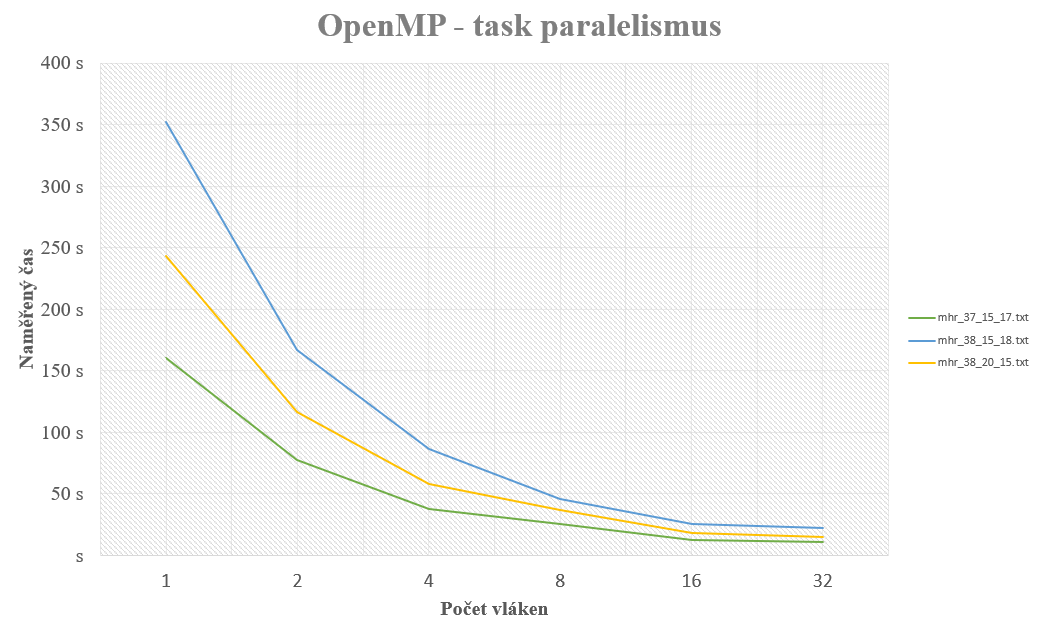
\includegraphics[width=\textwidth]{OpenMPtaskGraf.png}
\end{figure}

\noindent Následující graf znázorňuje efektivitu paralelního výpočtu u jednotlivých instancí problému pro jednotlivé počty výpočetních vláken.

\begin{figure}[H]
    \centering
    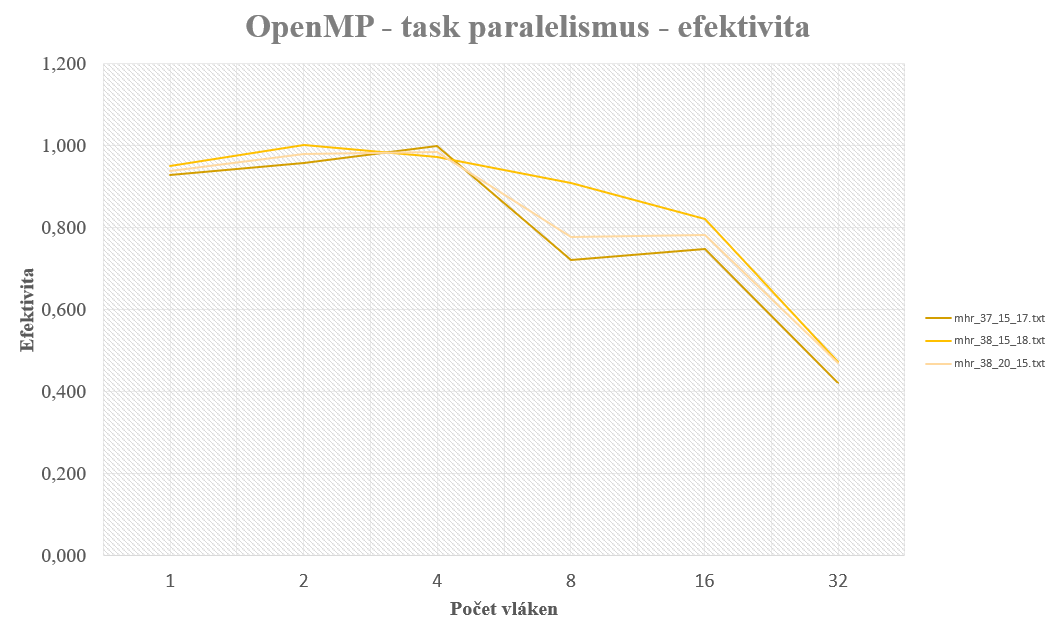
\includegraphics[width=\textwidth]{EfektivitaTask.png}
\end{figure}


\subsection{OpenMP řešení - datový paralelismus}
Následující tabulka obsahuje naměřené časy pro soubor \uv{mhr\_37\_15\_17.txt}:
\begin{table}[H]\centering
    \begin{tabular}{|c|c|c|c|}
        \hline \textbf{Počet vláken} & \textbf{Naměřený čas} & \textbf{Zrychlení} & \textbf{Efektivita} \\ \hline \hline
        1 & 154,4s & 0,964 & 0,964 \\ \hline
        2 & 77,2827s & 1,927 & 0,963 \\ \hline
        4 & 39,0135s & 3,817 & 0,954 \\ \hline
        8 & 21,6281s & 6,885 & 0,861 \\ \hline
        16 & 12,5573s & 11,858 & 0,741 \\ \hline
        32 &10,1305s & 14,699 & 0,459 \\ \hline
    \end{tabular}
\end{table} 
\noindent Následující tabulka obsahuje naměřené časy pro soubor \uv{mhr\_38\_15\_18.txt}:
\begin{table}[H]\centering
    \begin{tabular}{|c|c|c|c|}
        \hline \textbf{Počet vláken} & \textbf{Naměřený čas} & \textbf{Zrychlení} & \textbf{Efektivita} \\ \hline \hline
        1 & 316,323s & 1,059 & 1,059 \\ \hline
        2 & 156,825s & 2,135 & 1,068 \\ \hline
        4 & 79,3405s & 4,221 & 1,055 \\ \hline
        8 & 43,883s & 7,631 & 0,954 \\ \hline
        16 & 25,566s & 13,098 & 0,819 \\ \hline
        32 & 20,5225s & 16,317 & 0,510 \\ \hline
    \end{tabular}
\end{table} 

\noindent Následující tabulka obsahuje naměřené časy pro soubor \uv{mhr\_38\_20\_15.txt}:
\begin{table}[H]\centering
    \begin{tabular}{|c|c|c|c|}
        \hline \textbf{Počet vláken} & \textbf{Naměřený čas} & \textbf{Zrychlení} & \textbf{Efektivita} \\ \hline \hline
        1 &	222,581s & 1,025 & 1,025 \\ \hline
        2 &	111,741s & 2,041 & 1,021 \\ \hline
        4 &	48,0836s & 4,744 & 1,186 \\ \hline
        8 &	31,3636s & 7,273 & 0,909 \\ \hline
        16 & 17,2607s & 13,215 & 0,826 \\ \hline
        32 & 14,5187s & 15,711 & 0,491 \\ \hline
    \end{tabular}
\end{table} 

\noindent Graf níže znázorňuje zrychlení výpočtu jednotlivých instancí problému pro jednotlivé počty výpočetních vláken.

\begin{figure}[H]
    \centering
    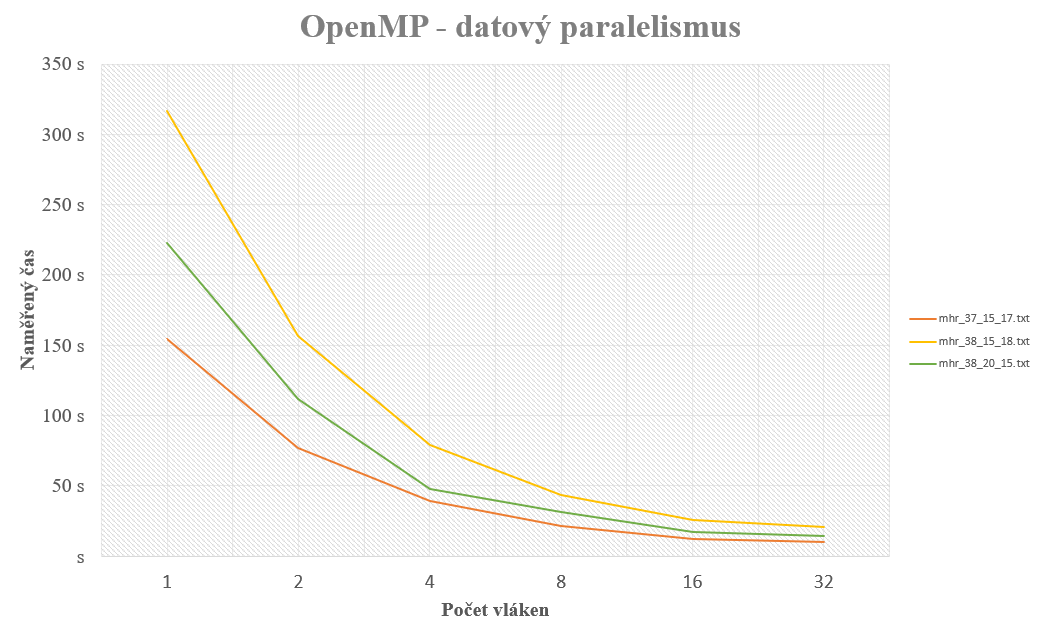
\includegraphics[width=\textwidth]{OpenMPdataGraf.png}
\end{figure}

\noindent Následující graf znázorňuje efektivitu paralelního výpočtu u jednotlivých instancí problému pro jednotlivé počty výpočetních vláken.

\begin{figure}[H]
    \centering
    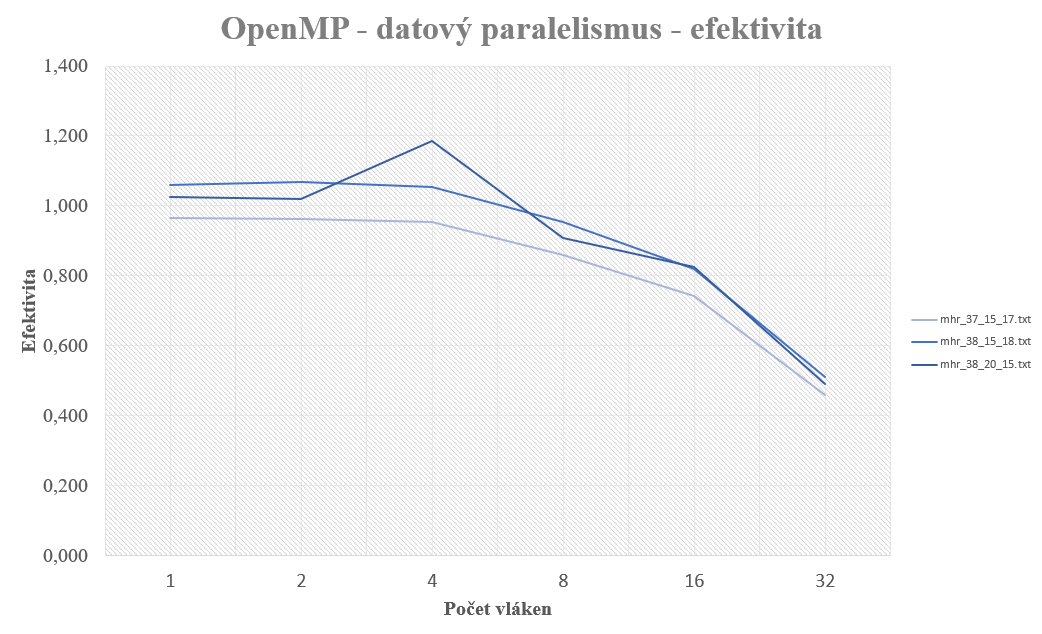
\includegraphics[width=\textwidth]{EfektivitaData.png}
\end{figure}

\subsection{MPI řešení}
Následující tabulka obsahuje naměřené časy pro soubor \uv{mhr\_37\_15\_17.txt}:
\begin{table}[H]\centering
    \begin{tabular}{|c|c|c|c|}
        \hline \textbf{Počet vláken} & \textbf{Naměřený čas} & \textbf{Zrychlení} & \textbf{Efektivita} \\ \hline \hline
        1 &	99,4959s & 1,497 & 1,497 \\ \hline
        2 &	50,5023s & 2,949 & 1,474 \\ \hline
        4 &	28,0085s & 5,317 & 1,329 \\ \hline
        8 &	16,1332s & 9,230 & 1,154 \\ \hline
        16 & 12,9762s & 11,476 & 0,717 \\ \hline
        32 &13,0327s & 11,426 & 0,357 \\ \hline
    \end{tabular}
\end{table} 
\noindent Následující tabulka obsahuje naměřené časy pro soubor \uv{mhr\_38\_15\_18.txt}:
\begin{table}[H]\centering
    \begin{tabular}{|c|c|c|c|}
        \hline \textbf{Počet vláken} & \textbf{Naměřený čas} & \textbf{Zrychlení} & \textbf{Efektivita} \\ \hline \hline
        1 &	169,494s & 1,976 & 1,976 \\ \hline 
        2 &	86,4336s & 3,874 & 1,937 \\ \hline
        4 &	47,9184s & 6,988 & 1,747 \\ \hline 
        8 &	27,5716s & 12,145 & 1,518 \\ \hline
        16 & 22,1723s & 15,103 & 0,944 \\ \hline
        32 & 22,2093s & 15,077 &0,471 \\ \hline
    \end{tabular}
\end{table} 

\noindent Následující tabulka obsahuje naměřené časy pro soubor \uv{mhr\_38\_20\_15.txt}:
\begin{table}[H]\centering
    \begin{tabular}{|c|c|c|c|}
        \hline \textbf{Počet vláken} & \textbf{Naměřený čas} & \textbf{Zrychlení} & \textbf{Efektivita} \\ \hline \hline
        1 & 139,421s & 1,636 & 1,636 \\ \hline
        2 &	70,8683s & 3,219 & 1,609 \\ \hline
        4 &	39,4595s & 5,781 & 1,445 \\ \hline
        8 &	22,8227s & 9,994 & 1,249 \\ \hline
        16 & 18,3458s & 12,433 & 0,777 \\ \hline
        32 & 18,4017s & 12,396 & 0,387 \\ \hline
    \end{tabular}
\end{table} 

\noindent Graf níže znázorňuje zrychlení výpočtu jednotlivých instancí problému pro jednotlivé počty výpočetních vláken.

\begin{figure}[H]
    \centering
    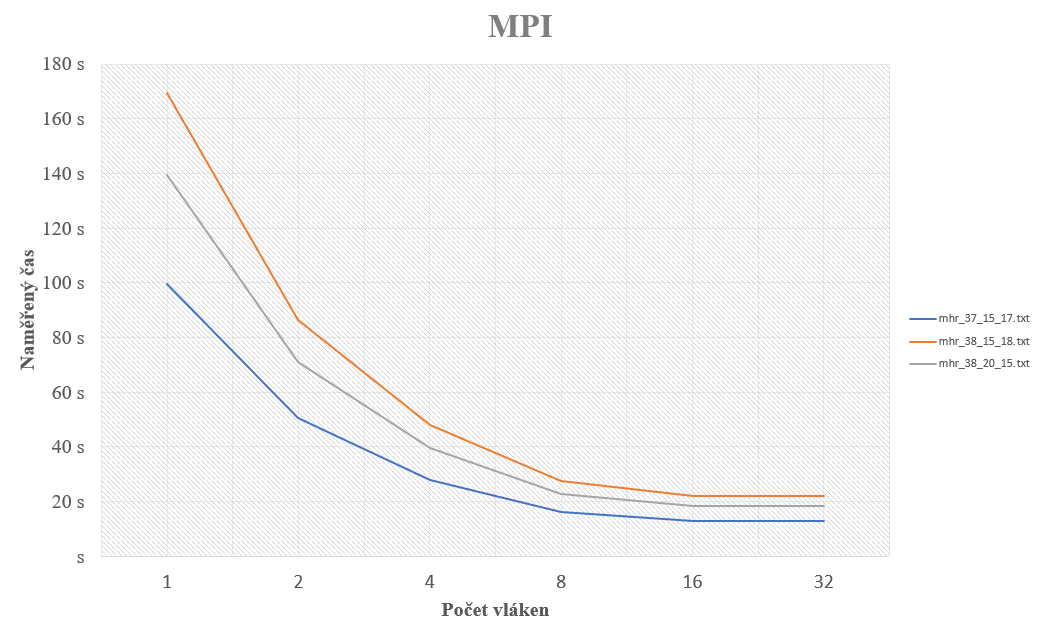
\includegraphics[width=\textwidth]{MPIGraf.png}
\end{figure}

\noindent Následující graf znázorňuje efektivitu paralelního výpočtu u jednotlivých instancí problému pro jednotlivé počty výpočetních vláken.

\begin{figure}[H]
    \centering
    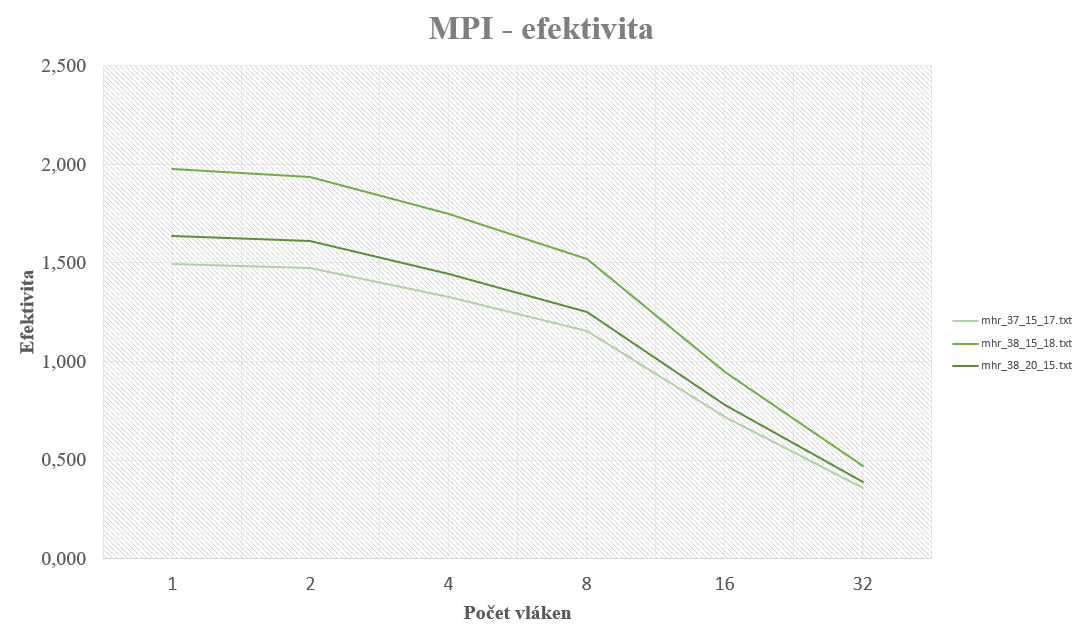
\includegraphics[width=\textwidth]{EfektivitaMPI.png}
\end{figure}

\subsection{Grafické porovnání algoritmů}

V této sekci jsou pomocí grafů znázorněna porovnání zrychlení a efektivity jednotlivých algoritmů. 

\begin{figure}[H]
    \centering
    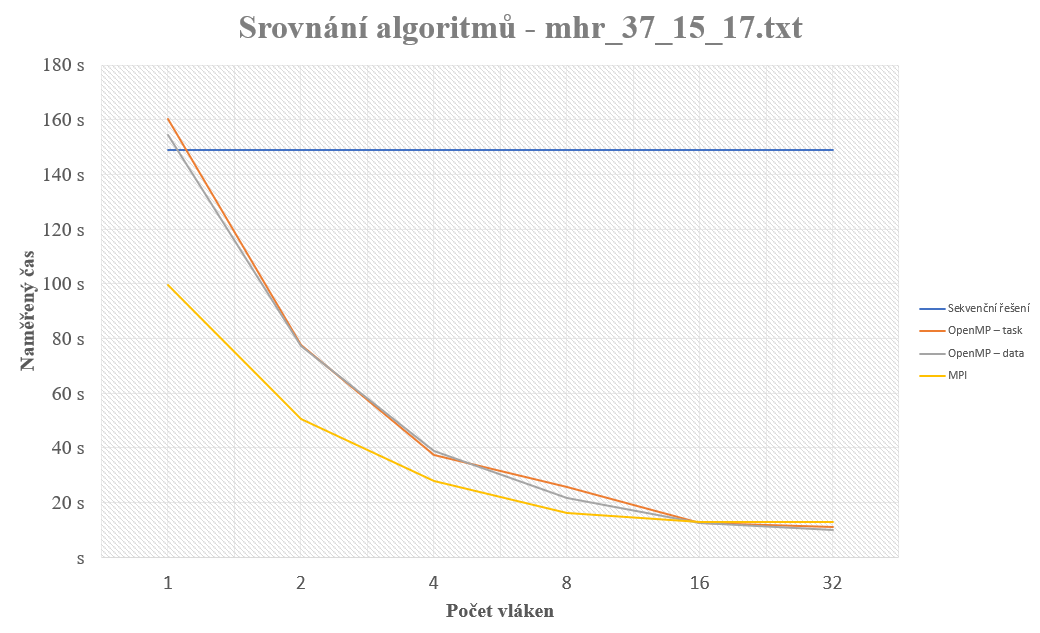
\includegraphics[width=\textwidth]{Srovnani371517.png}
\end{figure}
\begin{figure}[H]
    \centering
    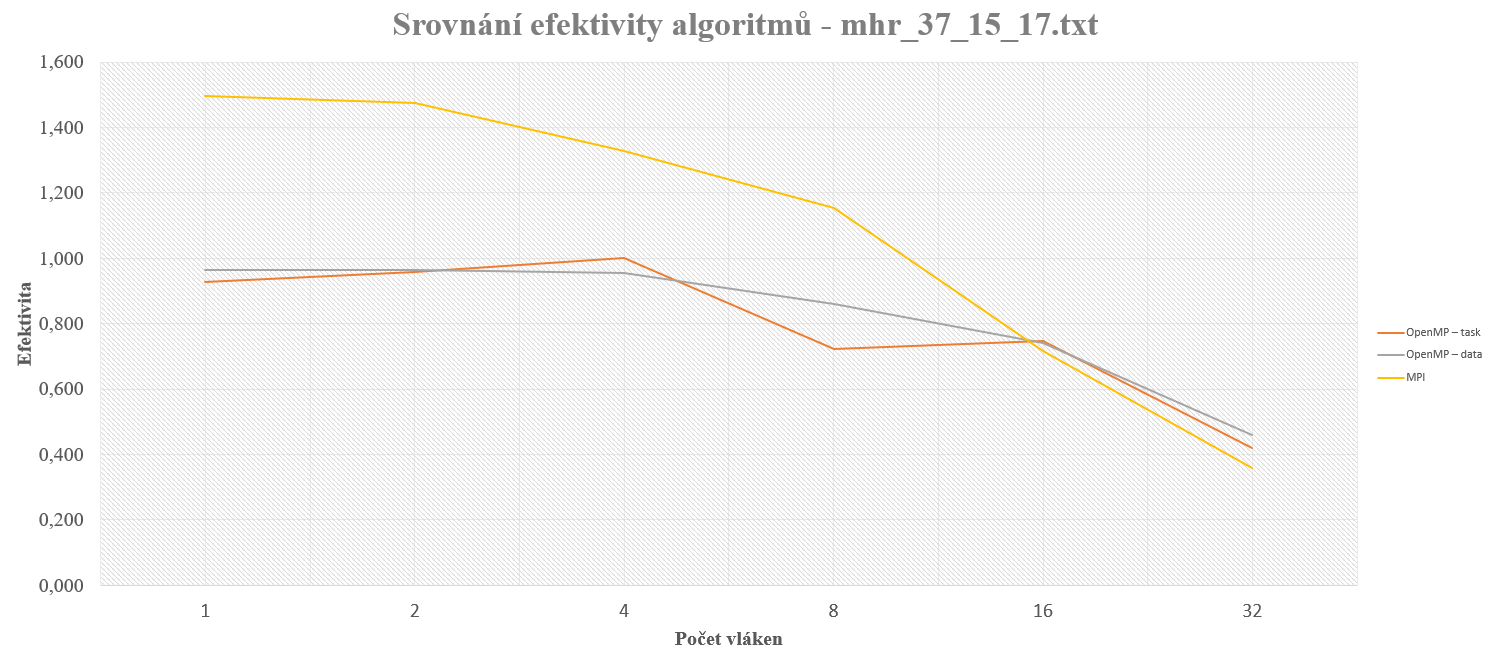
\includegraphics[width=\textwidth]{SE371517.png}
\end{figure}
\begin{figure}[H]
    \centering
    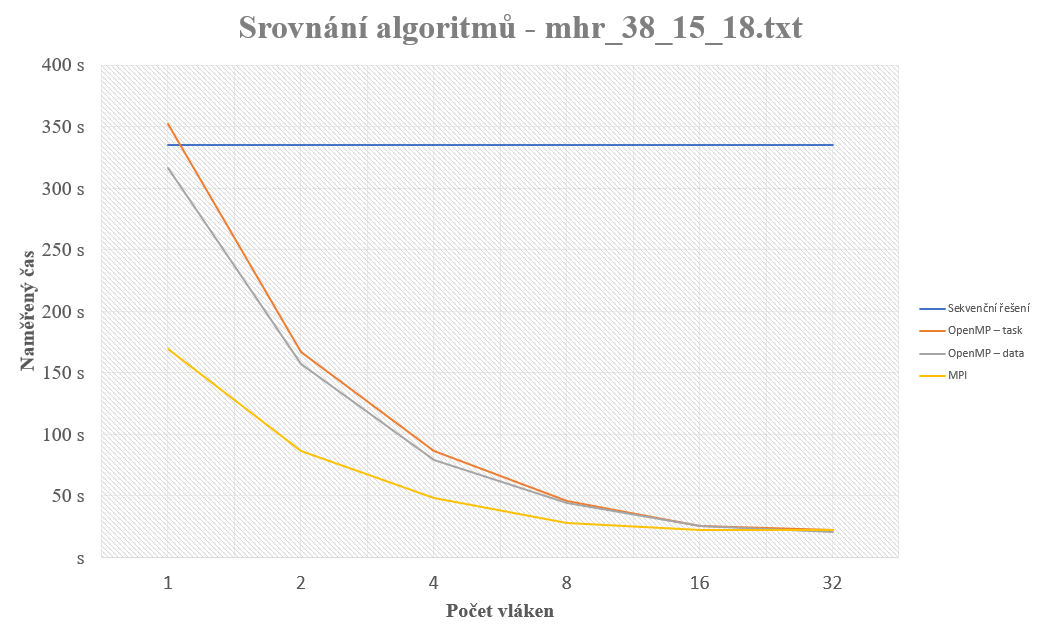
\includegraphics[width=\textwidth]{Srovnani381518.png}
\end{figure}
\begin{figure}[H]
    \centering
    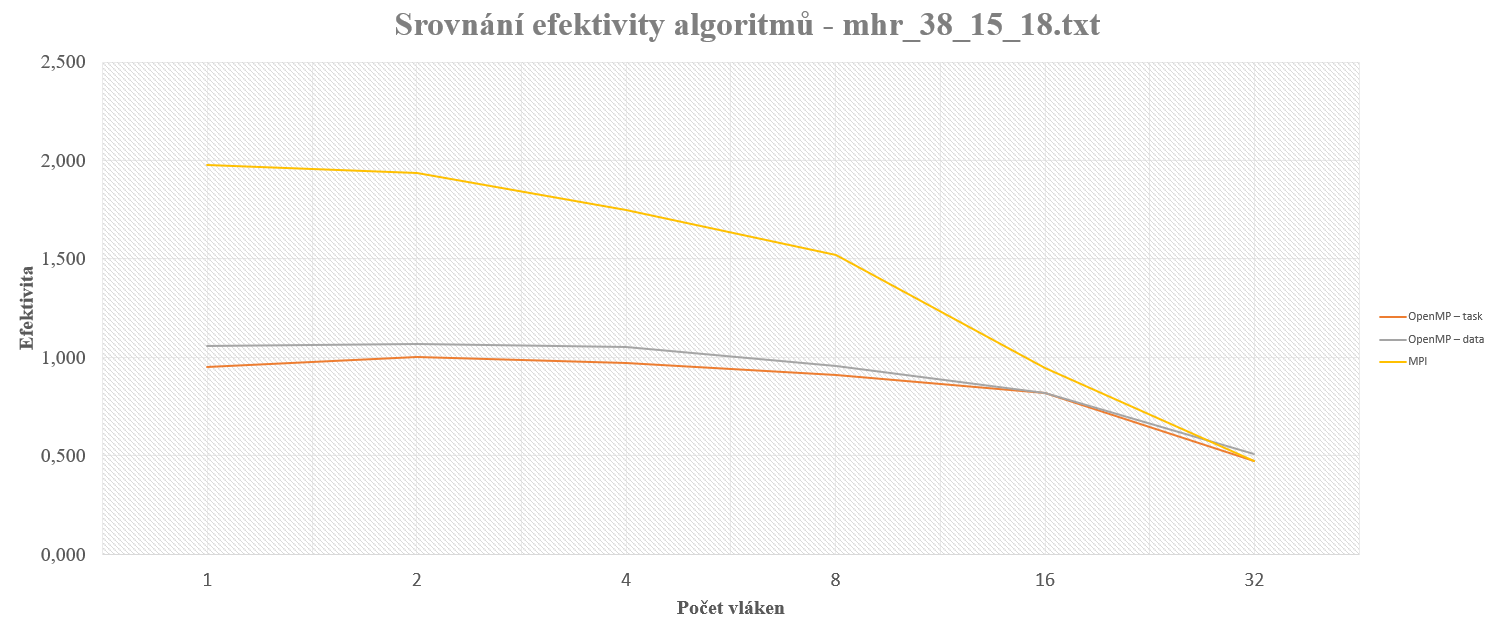
\includegraphics[width=\textwidth]{SE381518.png}
\end{figure}
\begin{figure}[H]
    \centering
    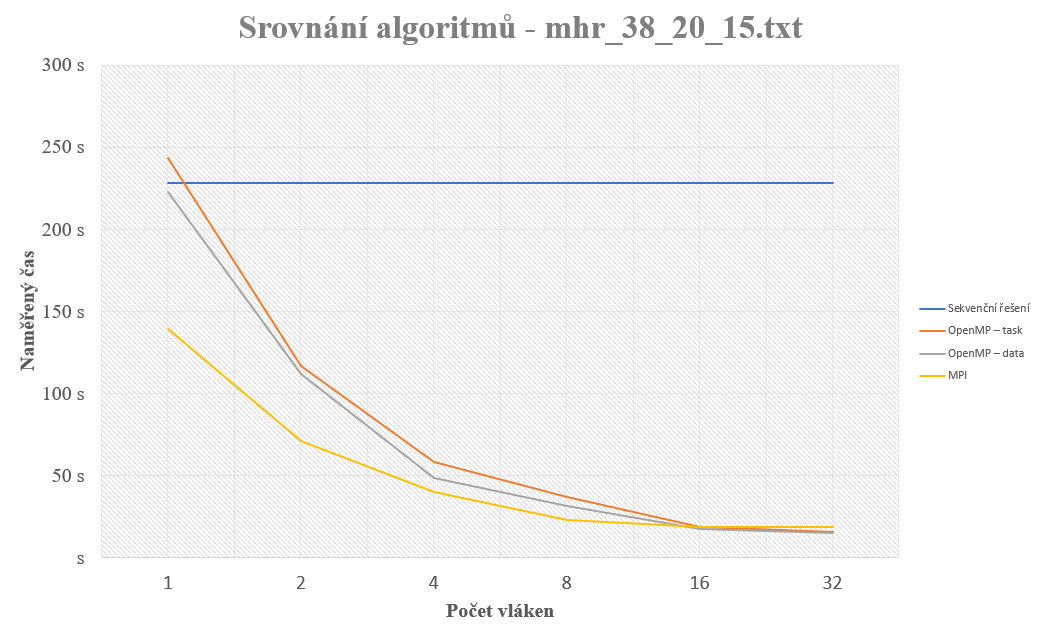
\includegraphics[width=\textwidth]{Srovnani382015.png}
\end{figure}
\begin{figure}[H]
    \centering
    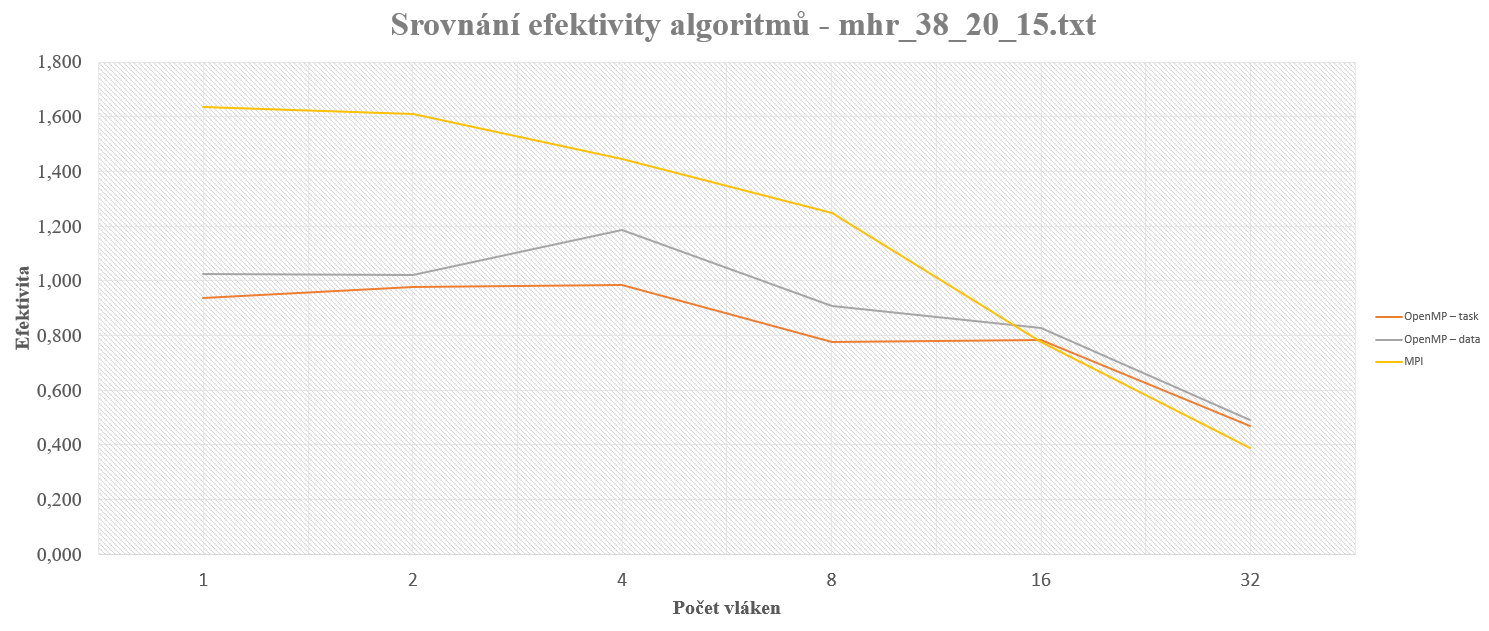
\includegraphics[width=\textwidth]{SE382015.png}
\end{figure}

\subsection{Analýza výsledků}
Z naměřených hodnot můžeme vypozorovat, že v některých případech jsme dokázali zrychlit sekvenční řešení až zhruba 16 krát. Dále si můžeme všimnout, že zrychlení výpočtu při přechodu z 16 na 32 vláken je ve většině případů zanedbatelné. Důvodem je skutečnost, že na fakultním klastru star, na kterém probíhala všechna měření, bylo k dispozici pro výpočet pouze 20 vláken. Dá se tedy očekávat, že jakýkoliv vyšší počet se na zrychlení běhu algoritmu nijak neprojeví. Pokud bychom však měli k dispozici více vláken (případně více procesů), mohli bychom dosáhnout ještě lepších výsledků. 

V případě OpenMP řešení jsme nejlepší hodnoty efektivity získali pro výpočty s 2 až 4 vlákny. V mnoha případech jsme dokonce dosáhli superlineáního urychlení. Pro MPI a obecně pro všechna měření platí, že efektivita s rostoucím počtem vláken ve většině případů klesá. Abychom zlepšili efektivitu, museli bychom zefektivnit paralelní výpočet, což už ale není moc možné.

Z grafů porovnání jednotlivých algoritmů je patrné, že MPI řešení dosahuje lepších hodnot zrychlení a~efektivity než OpenMP řešení v případě, že má dostatek vláken pro výpočet. V opačném případě jsou výsledky srovnatelné, možná dokonce mírně lepší u OpenMP řešení.

\section{Závěr}
Díky této práci a tomuto předmětu jsem si vyzkoušel návrh a implementaci paralelních algoritmů týkající se prohledávání stavového prostoru. Knihovny OpenMP a MPI jsou uživatelsky velmi přívětivé a nabízí obrovské možnosti paralelizace jednotlivých algoritmů. Pomocí kombinace těchto knihoven lze získat nejlepší výsledky na libovolně velkých výpočetních klastrech, aniž bychom k tomu potřebovali sdílenou paměť.

Celkově byl pro mě obrovský přínos vyzkoušet si tyto knihovny pro paralelizaci algoritmů v praxi a zjistit, jakých výsledků tyto algoritmy při využití knihoven OpenMP a MPI dosahují. Jednotlivé výsledky měření jsou zobrazeny a popsány v předchozí kapitole.

\section{Literatura}

[1] Stránka předmětu MI-PDP.16 na Courses: MI-PDP Paralelní a distribuované programování [online]. duben 2020, [cit.2020-04-30]. Dostupné z: \texttt{\href{https://courses.fit.cvut.cz/MI-PDP/index.html}{https://courses.fit.cvut.cz/MI-PDP/index.html}} \newline \newline
[2] Lísal, M.: Paralelní počítání. \textit{Ústí nad labem: Univerzita Jana Evangelisty Purkyně, Přírodovědecká fakulta}, 2006. ISBN 80-7044-784-2. 



\end{document}
